\section{Background}
\label{sec:background}

\subsection{SVE and SME Units on Arm CPUs}
\begin{figure}
    \centering
    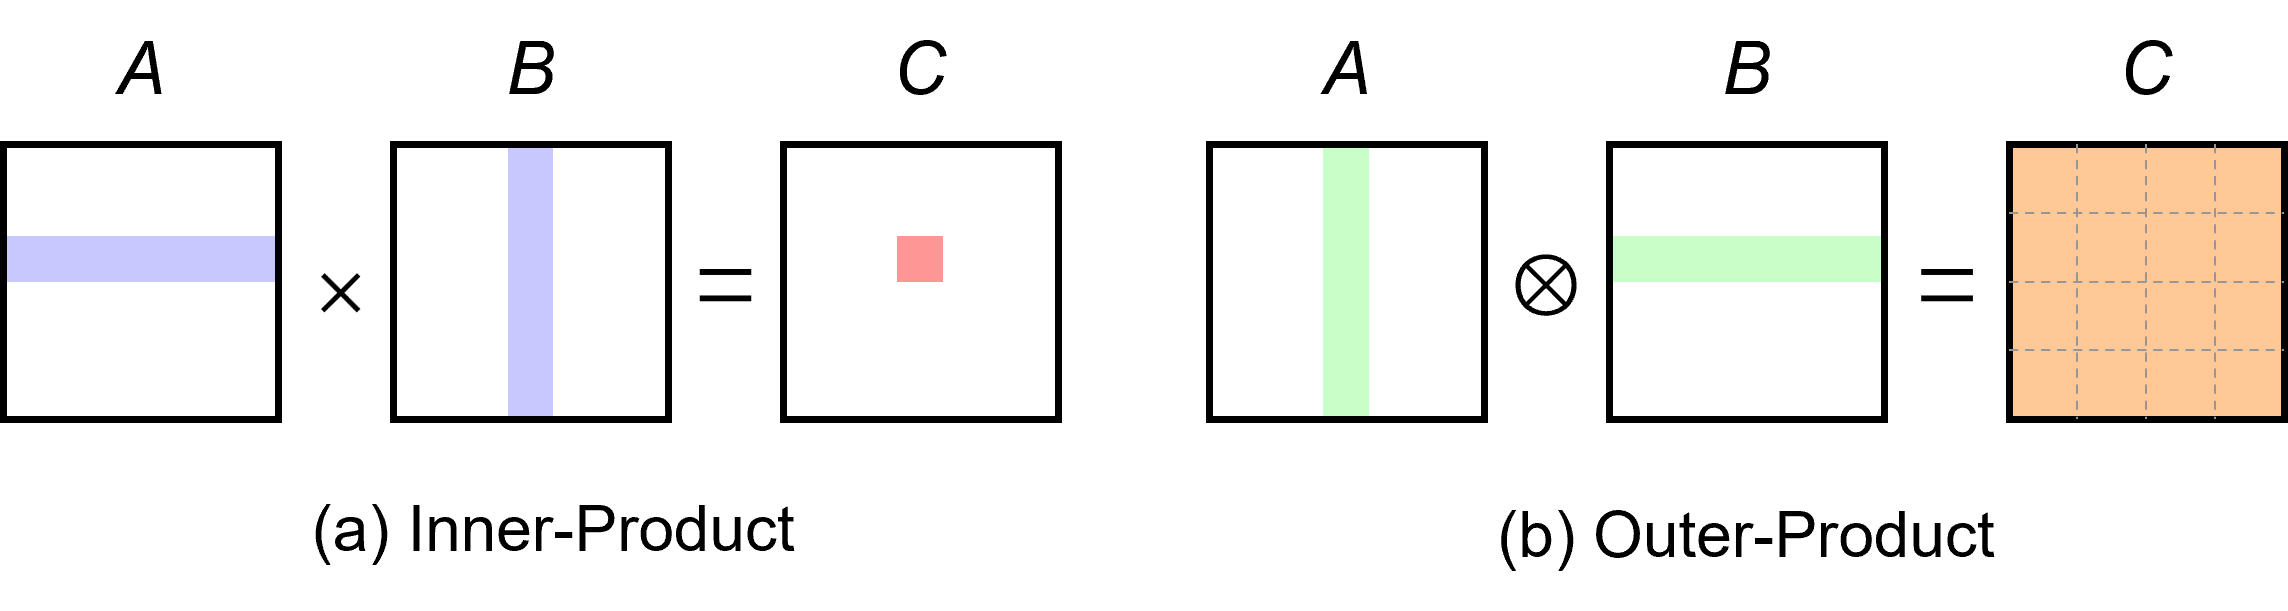
\includegraphics[width=0.95\linewidth]{figures/outerproduct.png}
    \caption{GEMM model of outer-product and inner-product.}
     \label{fig:outer_product_diagram}
\end{figure}

Arm processors have continuously expanded support for data-parallel and matrix-centric computation to satisfy increasing demand from HPC and AI workloads. Two architectural features, SVE and SME, are central to this trend. SVE provides a vector-length-agnostic SIMD model, while SME introduces a matrix-oriented outer-product execution model specialized for high-throughput accumulation (Figure~\ref{fig:outer_product_diagram}(b)). Understanding the execution semantics of these features is essential for the optimization of irregular GEMMs.

\textbf{SVE.} SVE~\cite{stephens2017arm} extends conventional SIMD through vector-length agnosticism. Instead of fixing vector width at compile time, SVE implementations expose vector lengths (VL) from 128 to 2048 bits in 128-bit increments. SVE also introduces predicate registers to control active lanes: each predicate element controls whether the corresponding lane is active, so inactive lanes are masked without control-flow divergence. This design handles loop tails and non-uniform trip counts efficiently without explicit scalar epilogues.

\textbf{SME.} SME builds on SVE and shifts the computational abstraction from lane-wise vectors to tile-wise accumulation. Architecturally, SME introduces the ZA matrix register file, a two-dimensional accumulator of $\mathit{VL} \times \mathit{VL}$ bytes that is logically partitioned into independent accumulator tiles. The number of tiles depends on element precision: element sizes of 1, 2, 4, 8, and 16 bytes correspond to 1, 2, 4, 8, and 16 tiles, respectively. Crucially, SME provides orthogonal access to ZA, allowing tiles to be read or written by either rows or columns without explicit data rearrangement. This eliminates software-level transposition and improves data reuse across tensor dimensions.

Computation in SME is driven by a hardware outer-product unit. Given a horizontal source vector $u$ and a vertical source vector $v$, the MOPA instruction computes their outer product and accumulates the result into a destination tile $D$:
$$
    D \leftarrow D + (u \otimes v).
$$
A single MOPA delivers $O(\mathit{VL}^2)$ operations and contributes a rank-1 update to the tile; repeated updates along the reduction dimension construct the final tile entirely in ZA. Because partial sums remain in ZA across many instructions, pressure on general vector registers is reduced and arithmetic intensity is much higher than what SVE alone can achieve.

For reduced-precision workloads, SME employs widening outer-product operations in which lower-precision inputs are multiplied and accumulated into wider-precision tiles. For example, FP16 inputs are accumulated into FP32 tiles via a two-way accumulation (pairs of adjacent FP16 elements are multiplied independently and summed into one FP32 element of the tile), preserving numerical robustness while increasing throughput compared with FP32 execution.

These benefits come with structural constraints. The efficiency of SME depends on matching problem dimensions with tile geometry, and the overhead of ZA data movement must be amortized by sufficient computation. Therefore, applying SME to irregular GEMMs---such as the tall-and-skinny shapes that dominate AlphaFold2---demands specialized optimization strategies to prevent severe performance degradation.

\subsection{The Architecture of 920F CPU}
% \subsection{The Architecture of 920F CPU}
% 920F CPU提供了OPA(Outer-Product Accumulator)以及配套的向量指令用于加速矩阵计算。920F使用一个array register来存储外积计算的结果，该array register可以被拆分为1个8-bits元素、2个16-bits元素、4个32-bits元素或8个64-bits元素的寄存器。对于每种数据类型，array register均含有VL(vector lenght) $\times$ VL个元素。OPA指令从将两个向量寄存器中的向量做外积，并累加到相应精度的array register上。920F 提供了int8、fp16、fp32、fp64的OPA指令。int8的OPA指令会将输入寄存器划分为4个向量，并在int32精度的array register上累加4组外积的结果。fp16的OPA指令会将输入寄存器划分为两个向量，并在fp32精度的array register上累加2组外积的结果。fp32与fp64则是直接在相应精度的array register上累加一组外积的结果。对于fp16(int8)的OPA指令，920F要求同一个输入寄存器内的向量是交织的，也即每个外积向量的元素索引之差为2(4)。

\begin{figure}[t]
    \centering
    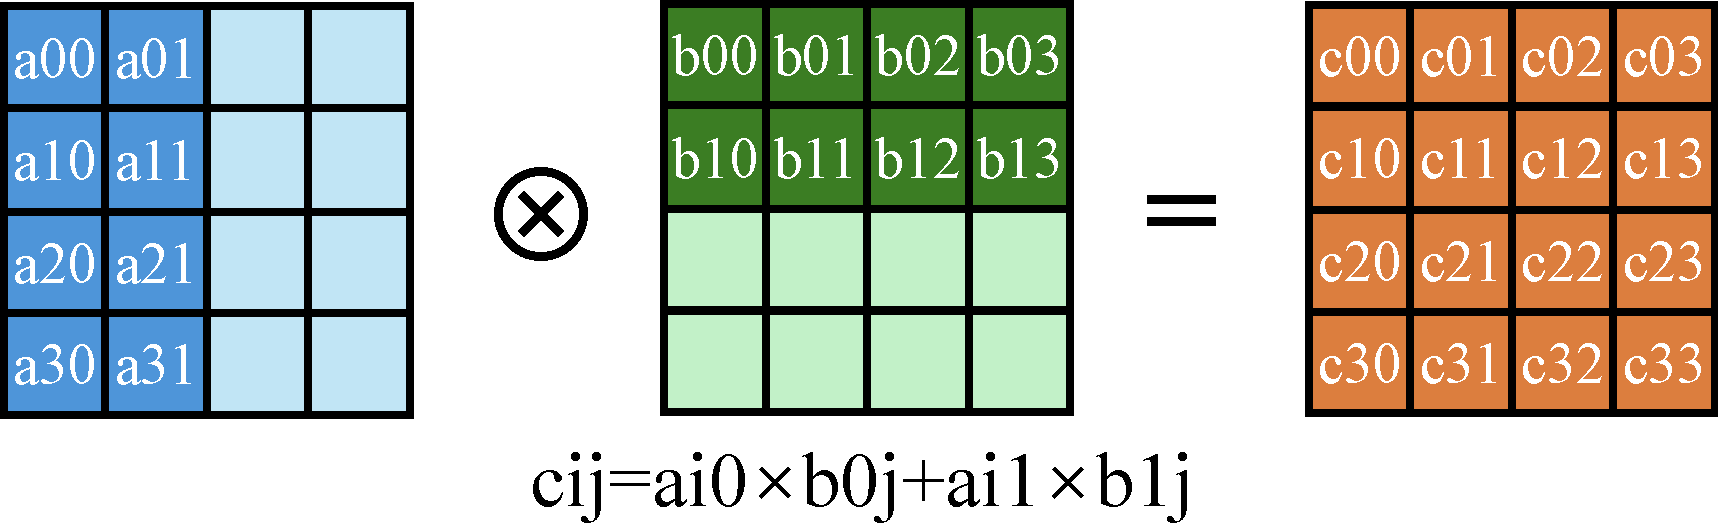
\includegraphics[width=0.8\linewidth]{figures/opa_2way.pdf}
    \caption{2-way OPA Instruction on 920F CPU.}
    \label{fig:opa}
\end{figure}

The 920F processor is a representative many-core ARM CPU that implements the SME extension described above. As a concrete instance of an outer-product-accumulator (OPA) architecture, it inherits the ZA matrix register file and MOPA-style execution semantics, while adding several platform-level characteristics that shape its performance profile.

\textbf{Many-core multi-NUMA organization.} A single 920F socket integrates more than 256 cores partitioned into 8 NUMA domains, with each core exposing its own per-core SME unit. The processor further provides high-bandwidth on-package memory and a dedicated memory movement unit for hardware-assisted bulk transfers. These features allow large activation tensors to remain on-package, which is particularly valuable for AlphaFold2 inference, but also introduce non-uniform access costs that must be managed by the software.

\textbf{Vector length and supported precisions.} The 920F implements a 512-bit vector length (VL = 512), so each ZA tile holds $64 \times 64$ FP16 elements or $16 \times 16$ FP32 elements after the standard precision-based partitioning. Native MOPA instructions are provided for FP32, FP16, and INT8 inputs. In this work, we focus on FP32 and FP16 computation modes.

\textbf{Two-way FP16 OPA.} As a concrete instantiation of the widening outer product, Fig.~\ref{fig:opa} illustrates the 2-way FP16 MOPA on 920F: each input vector register is interpreted as two interleaved sub-vectors of FP16 elements, and one instruction accumulates two FP16 outer products into a single FP32 destination tile. This interleaved operand layout is a hardware requirement: when the source data is stored row-major in memory, an explicit reinterpretation step is needed before the OPA can consume it. Section~\ref{sec:optimizations} discusses how we exploit ZA's orthogonal row/column access to perform this reinterpretation with minimal overhead.

% For quantized integer inference, the architecture leverages the reduced bit-width to perform a \textit{4-way outer product} ($K=4$), as illustrated in Fig.~\ref{fig:opa}.
% When operating on 8-bit integer (INT8) data, the source vectors are processed as groups of four consecutive elements. The hardware computes the outer product of a 4-element sub-vector from the row input and a 4-element sub-vector from the column input, accumulating the sum into a 32-bit integer (INT32) destination tile. By packing four 8-bit multiplications into a single accumulator update, this 4-way mechanism significantly increases the arithmetic intensity and allows for efficient utilization of the available memory bandwidth.



% \subsection{Mixed Precision Model Inference}
% Model quantization is a widely adopted technique in deep learning that reduces the precision of model parameters and intermediate activations to improve inference efficiency.~\cite{krishnamoorthi2018quantizing,polino2018model,jacob2018quantization} Instead of relying solely on high-precision floating-point formats such as FP32 or FP16, quantization typically converts data into lower-bit integer formats (e.g., INT8). This reduction not only decreases the memory footprint and data transfer volume but also allows hardware accelerators, including CPU matrix units, to perform more operations per cycle due to higher arithmetic density.

% % Quantization methods can be broadly categorized into two groups: post-training quantization (PTQ) and quantization-aware training (QAT). PTQ directly converts a pre-trained floating-point model into a lower-precision version, often requiring minimal additional computation. While PTQ is attractive for deployment, it may suffer from accuracy degradation, particularly for models with sensitive numerical operations. In contrast, QAT simulates quantization effects during training, enabling the model to adapt to low-precision arithmetic. This usually yields higher accuracy but requires additional training resources.

% Recent advances in quantization have demonstrated that many large-scale deep learning models in computer vision and natural language processing can be effectively quantized to INT8 with negligible accuracy loss. Furthermore, modern hardware platforms, including CPUs with specialized matrix units, provide native support for integer arithmetic, making quantization a natural fit for high-performance inference on general-purpose processors.

% However, applying quantization to AlphaFold2 introduces unique challenges. The model integrates heterogeneous computations, ranging from long-sequence attention to triangular updates and geometric transformations. These operations are not only memory-intensive but also highly sensitive to numerical precision. Small rounding errors during quantization can propagate and amplify through iterative refinement, potentially leading to distorted protein structures. Therefore, careful design of quantization strategies, including operator-level calibration, mixed-precision schemes, and error-compensation techniques, is essential to maintain prediction accuracy while benefiting from the efficiency of low-precision execution.

% \subsection{Statistics of AlphaFold2}
% \begin{figure*}[htbp]
%     \centering
%     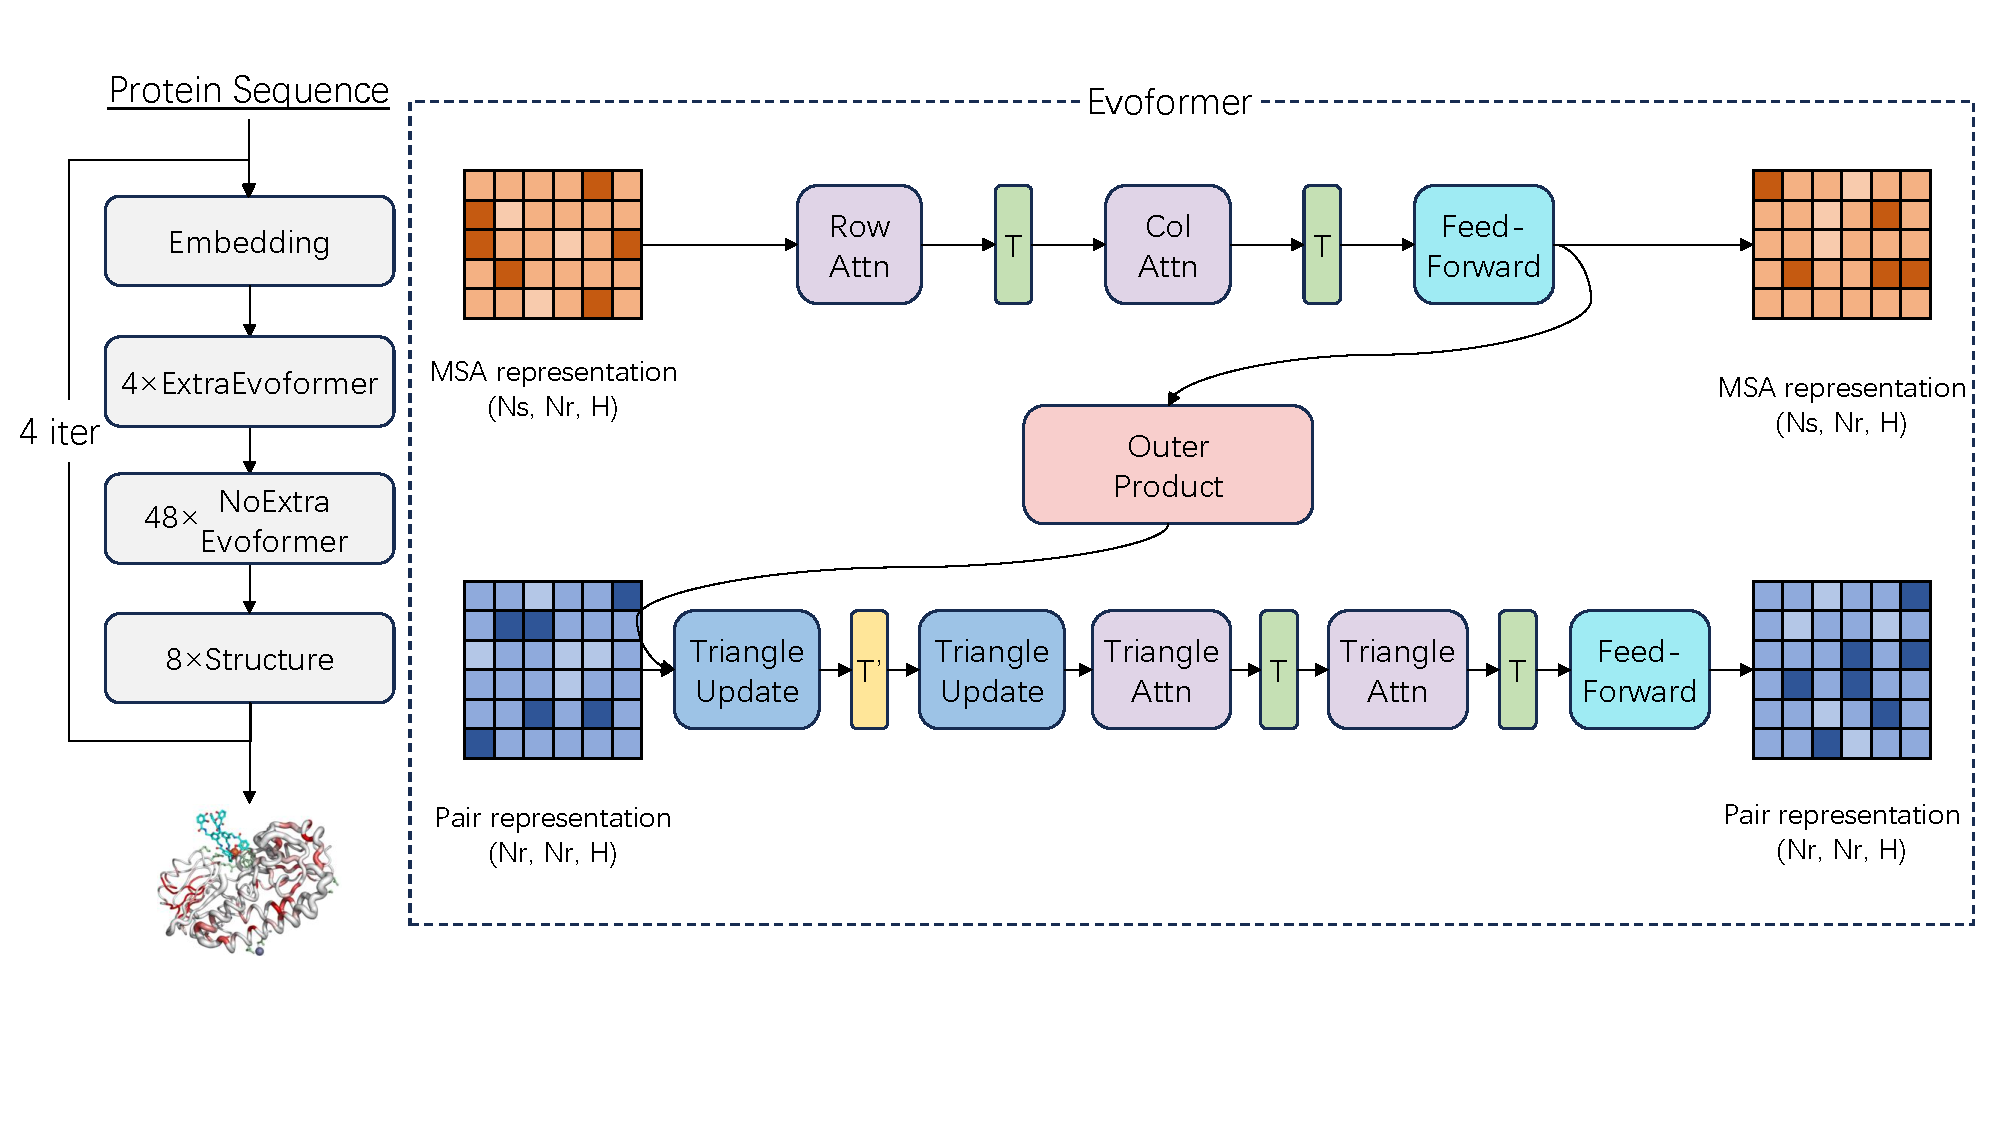
\includegraphics[width=\textwidth]{figures/AlphaFold.pdf}
%     \caption{AlphaFold2 Model Architecture}
%     \label{fig:af2model}
% \end{figure*}
% % AlphaFold2 adopts a highly modular architecture that integrates multiple neural network components to capture both local sequence features and long-range structural dependencies. The overall pipeline can be divided into three main stages: the Embedding Module, the Evoformer and the Structure Module.

% % The Evoformer is the central component that processes two key data representations: the multiple sequence alignment (MSA) features and pairwise residue features. It employs a combination of transformer blocks, attention mechanisms, and triangular multiplicative updates to model evolutionary relationships and inter-residue interactions. This stage is both compute- and memory-intensive, as it involves long-sequence attention operations and large tensor transformations.

% % The Structure Module takes the processed representations from the Evoformer and generates three-dimensional protein structures. It employs a recurrent geometry-based update procedure that iteratively refines atomic coordinates, ensuring that predicted conformations are physically consistent. This module involves numerous rigid-body transformations and specialized operations on rotation and translation groups, which differ from conventional deep learning layers.

% % Finally, AlphaFold2 relies on iterative refinement, where the Evoformer and Structure Module are applied multiple times to progressively improve prediction accuracy. This iterative nature further amplifies the computational demands of the model.

% AlphaFold2 has established a new paradigm in protein structure prediction by integrating deep learning with evolutionary and physical constraints. Given an amino acid sequence, AlphaFold2 predicts the three-dimensional atomic structure with an accuracy comparable to experimental methods such as X-ray crystallography~\cite{smyth2000x} and cryo-EM~\cite{bai2015cryo,earl2017cryo}. This breakthrough has had a profound impact on structural biology, drug discovery, and protein engineering, while also drawing significant attention from the computer systems community due to its computational complexity.

% As shown in Fig.~\ref{fig:af2model},
% AlphaFold2 consists of three major stages: input representation, Evoformer, and structure module.

% \textbf{Input representation.} The model first extracts features from the target protein sequence and its multiple sequence alignment (MSA). This process produces two key embeddings: a per-residue sequence embedding and a pairwise embedding that encodes residue-residue relationships.

% \textbf{Evoformer.} This stage is the computational core of AlphaFold2 and accounts for the majority of runtime and memory usage. The Evoformer is a deep stack of transformer-like blocks that iteratively refines both the MSA embedding and the pairwise embedding. Unlike standard NLP transformers, the hidden dimensions in AlphaFold2 are relatively small (typically 128 or 256), which means the memory footprint of model weights is modest. Instead, the memory bottleneck comes from activations, especially when processing long protein sequences, where both the MSA and pairwise representations can grow quadratically. Moreover, \textit{logits} in these modules exhibit cubic growth. Another distinctive feature is that the Evoformer alternates between intra-chain attention (within a single protein chain) and inter-chain attention (across multiple chains). These modules require frequent reshaping of data layouts. As a result, activation tensors are repeatedly transposed between different memory layouts, introducing additional communication overhead.

% \textbf{Structure module.} Using the refined representations, the structure module predicts 3D atomic coordinates. It relies on geometric reasoning over rotations and translations, converting pairwise features into structural constraints. Compared to the Evoformer, this stage is relatively lightweight in terms of computation, but essential for ensuring physically plausible predictions.

% From a systems perspective, AlphaFold2 exhibits several properties that distinguish it from typical deep learning workloads.

% \textbf{Activation-dominated memory footprint.} In contrast to large NLP models, AlphaFold2 has relatively small hidden dimensions, and thus, the memory contribution of model weights is minor. Instead, the dominant memory cost arises from activations, particularly for long sequences, where both MSA and pairwise representations scale with sequence length.

% % \textbf{Frequent communication due to tensor transpositions.} To enforce the physical plausibility of the protein structure, AlphaFold2 interleaves different types of attention and pairwise updates, many of which require switching tensor layouts. For example, intra-chain and inter-chain attention operate on different axes of the same tensor, leading to repeated transpose operations. These data movements create significant communication overhead, especially on architectures where cross-NUMA transfers are expensive.In Fig.~\ref{fig:af2model}, the transposition is denoted by \textit{T}, and \textit{T'} represents an equivalent transposition operation.

% \textbf{Dense linear algebra as the dominant computation.} Similar to other transformer-based models, AlphaFold2 is heavily dominated by matrix multiplications and other dense tensor operations, making it highly dependent on the efficiency of GEMM kernels and memory bandwidth.

% The activation-heavy memory usage, and dense linear algebra kernels together make AlphaFold2 both compute- and memory-intensive. In the next section, we present a detailed bottleneck analysis to quantify these challenges and identify the optimization opportunities for the 920F CPU.

% % From a systems perspective, AlphaFold2 presents several unique challenges compared to conventional vision or language models. First, its extensive use of attention across long MSAs leads to quadratic computational complexity with respect to sequence length. Second, the triangular updates and geometric transformations require substantial matrix multiplications interleaved with non-standard operations, making the workload heterogeneous and difficult to optimize. Third, the model's memory footprint is significant, as it maintains multiple high-dimensional feature tensors across iterations. These characteristics make AlphaFold2 particularly demanding for hardware platforms and motivate careful exploration of architectural accelerators such as matrix units on CPUs.
